\subsubsection{Target}
Il segmento di mercato al quale \NOMEPROGETTO{} si rivolge è costituito dalla nicchia di mercato rappresentata da un utenza business, la quale ha la necessità di catalogare con precisione e senza perdite di tempo, le numerose newsletter che quotidianamente giungono alla casella di posta elettronica.\\
Nello specifico si vogliono raggiungere i \emph{liberi professionisti} quali avvocati, architetti, ingegneri, ma anche \emph{imprenditori} di PMI che spesso gestiscono personalmente un account di posta.\\
Tutti questi soggetti hanno la necessità di gestire con efficienza le email ma spesso non hanno il tempo necessario per farlo in modo efficace: \NOMEPROGETTO{} riesce a colmare esattamente questa lacuna rendendo ogni operazione intuitiva ed immediata.
Si possono quindi delineare 3 segmenti di target diversi che riscontrano problematiche simili ma con soluzioni leggermente diverse:
\begin{description}
\item[Liberi professionisti:] segmento a cui appartengono le più svariate categorie di lavoratori freelance; tra questi si possono trovare architetti, ingegneri, commercialisti, medici, avvocati, consulenti in diversi ambiti.\footnote{\url{http://it.wikipedia.org/wiki/Libero\_professionista}}\\
Questi sono persone che lavorano in autonomia e devono gestire personalmente la posta in arrivo, sia che essa sia di clienti, sia che riguardi newsletter a cui il professionista è iscritto. Probabilmente un singolo lavoratore possiede più indirizzi email e questo contribuisce a complicare ulteriormente la gestione corretta della posta.\\
Questo segmento è quindi interessato ad un prodotto di semplice utilizzo, efficiente ed affidabile e capace di gestire diversi account di posta anche in mobilità.
\item[Studi privati:] questo segmento identifica professionisti che, diversamente dalla categoria precedente, hanno aperto uno studio nel quale lavorano a stretto contatto con un ristretto numero di soci e dipendenti\footnote{\url{http://it.wikipedia.org/wiki/Piccola\_e\_media\_impresa}}; appare evidente come la presenza di più persone con i relativi contatti email personali, stia ad indicare una maggiore necessità di controllo del traffico della posta, in quanto i volumi saranno maggiori rispetto ad un singolo utente.\\
Di conseguenza il prodotto più adatto per questa categoria deve essere in grado di fornire una gestione centralizzata degli account e dei servizi di condivisione delle informazioni.\\
\item[PMI:] le piccole e medie imprese presentano caratteristiche ancora diverse dalle 2 categorie precedenti, in primo luogo perché hanno una struttura organizzativa aziendale con una netta divisione dei compiti; la visione della posta sarà quindi una mansione affidata a determinate categorie di dipendenti i quali possono non essere direttamente interessati alle newsletter in entrata: appare quindi fondamentale che i diretti interessati possano avere modo di accedere a tali informazioni in modo agevole e completo.\\
Il prodotto software deve essere quindi in grado di gestire un database di discrete dimensioni accedibile da più persone anche contemporaneamente, deve quindi avere doti di robustezza e affidabilità notevoli, nonchè reattivo alle richieste che vengono effettuate.
\end{description}

\subsubsection{Competitors}
Per approfondire la conoscenza del mercato dei software di gestione delle email si è resa necessaria una ricerca approfondita dei possibili competitors presenti nel panorama internazionale, in modo da comprendere al meglio i pregi e i difetti di tali soluzioni per poter implementare caratteristiche innovative e peculiarità uniche tali da rendere \NOMEPROGETTO{} un prodotto unico nel suo genere.

\paragraph{G-lock Email Processor} 
\url{http://www.glocksoft.com/email-processor}

\begin{figure}[H]
\centering
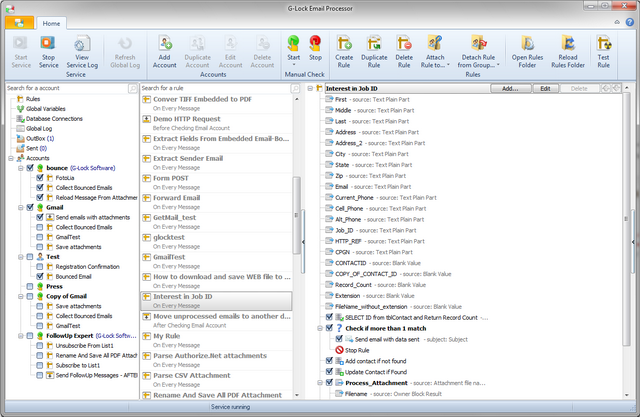
\includegraphics[scale=0.5]{img/gep-main-window-1.png}
\caption{Schermata G-Lock Email Processor}
\end{figure}

Il software è in grado di:
\begin{itemize}
\item Controllare automaticamente l'account di posta in modo regolare ed elaborare i messaggi in background;
\item Convertire il contenuto del messaggio in record di database;
\item Salvare i dati estratti dal messaggio in un file;
\item Salvare gli allegati dei messaggi sul disco;
\item Creare un report in formato PDF o HTML;
\item Integrare i dati estratti in Microsoft Outlook;
\item Ottimizzare il proprio business ed il servizio al cliente con l'invio di risposte automatiche;
\item Convertire automaticamente i dati estratti utilizzando MS Windows script;
\item Estrarre URL da e-mail e processare dati da pagine web e feed RSS;
\end{itemize}

\begin{figure}[H]
\centering 
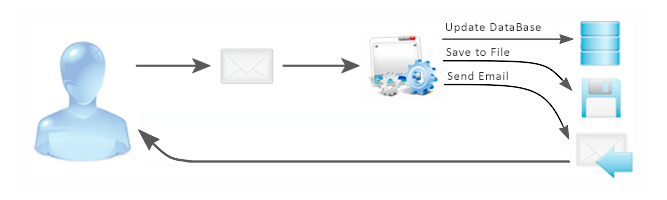
\includegraphics[scale=2]{img/emailprocessor.png} 
\caption{Funzionalità G-Lock Email Processor}
\end{figure}

Il software si presenta come la migliore soluzione trovata sul mercato ma possiede alcuni importanti difetti: è compatibile solamente per la piattaforma Microsoft Windows, il quale ricopre un'ampia fetta di mercato ma non la totalità, e il prezzo è considerevolmente alto per una singola licenza, 295 USD.
\newpage

\paragraph{Email2db}
\url{http://www.email2db.com/email-to-database.aspx}

\begin{figure}[H]
\centering 
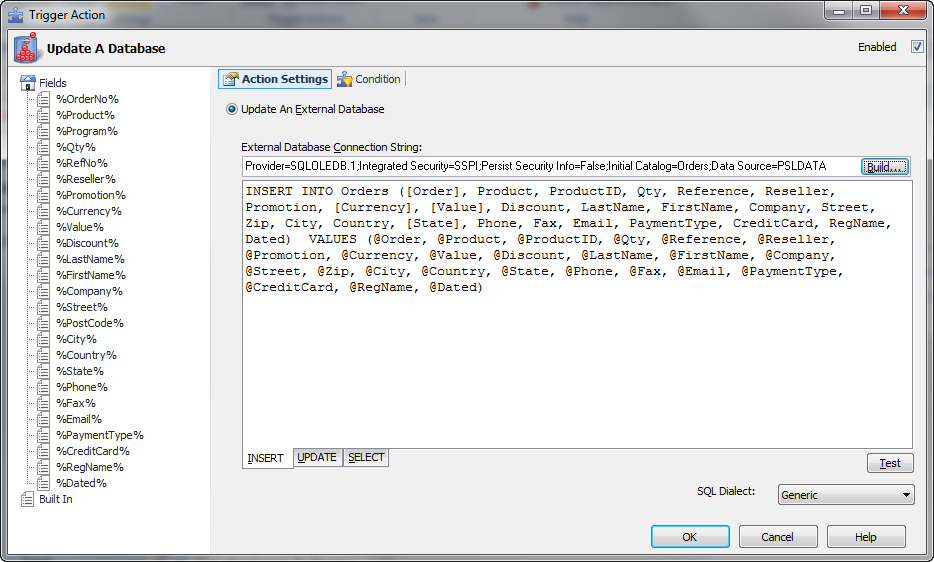
\includegraphics[scale=0.6]{img/email2db.png} 
\caption{Schermata Trigger Email2db}
\end{figure}

Email2DB è uno strumento per l'automazione di messaggi che è possibile utilizzare per convertire email e altri tipi di messaggi in record per database ed inoltre permette di convertire qualsiasi forma di messaggio anche in formato Excel o in record CSV.

Il software è grado di:
\begin{itemize}
\item i leggere messaggi e-mail provenienti da più fonti (server POP3, server IMAP, server Exchange, feed di Twitter, pagine Web, feed RSS e database esterni);
\item creare un numero qualsiasi di trigger. Il trigger è un insieme di condizioni che Email2DB verifica (per esempio, uno specifico mittente o parole specifiche nell'oggetto). Se un messaggio supera le condizioni del trigger, Email2DB elabora una serie di azioni su di esso. Queste azioni comprendono l'aggiornamento di una banca dati, l'invio di eventuali risposte e-mail e report di stampa;
\item analizzare ed estrarre dati da e-mail e aggiornare diversi tipi di database, tra cui SQL Server, MySQL, Oracle, Pervasive, Access e qualsiasi altro database che supporti ADO o ODBC;
\item salvare i dati su foglio di calcolo Excel o file CSV.
\end{itemize}

Email2DB è disponibile in diverse versioni: Small Business, Enterprise, Data Center \& Developer.\\
Tutte le edizioni includono le stesse funzionalità per l'analisi e l'estrazione di dati da e-mail per aggiornare più database, permettono di gestire un numero illimitato di account e trigger per l'elaborazione.\\
Inoltre tutte le edizioni non hanno restrizioni sul tipo di messaggi che possono analizzare (Server POP3, IMAP, feed di Twitter) ma per esempio solo le versioni Enterprise e Developer permettono di spostare il messaggio corrente in una cartella diversa da quella in cui è arrivato.

Anche per questo software sorge lo stesso problema del precedente in quando è utilizzabile solo su piattaforme Windows 7/8, Vista, XP, 2003 Server, 2008 Server, 2012 Server.\\
Il software è a pagamento con un costo a partire da 475\euro per l'edizione Small Business, 995\euro per quella Enterprise, 475\euro per quella Developer e 3195\euro per la Data Center Edition, ma permette una prova gratuita di 30 giorni dopo essersi registrati.

\subsubsection{Valore aggiunto}
Dall'analisi dei competitors è emerso come non esista sul mercato un software \emph{multipiattaforma} che soddisfi i bisogni riscontrati nel capitolato; questa è una notevole mancanza in quanto non esiste solo il mondo Microsoft, anzi il mercato dei sistemi operativi sta andando incontro a notevoli cambiamenti, soprattutto con l'avvento dei terminali mobile e di Android; risulta evidente come non basta più coprire la fetta maggiore di pubblico, ma è necessario rendere il prodotto fruibile alla maggior parte delle persone e dei dispositivi.

\subsubsection{Distribuzione prodotto}

\subsubsection{Promozione prodotto}